\documentclass{article}
\usepackage[utf8]{inputenc}
\usepackage{amsmath}
\usepackage{graphicx}
\graphicspath{ {./images/} }

\title{CS 224n Assignment 2: word2vec}
\author{Chrysa Dikonimaki}
\date{August 2020}

\renewcommand{\thesubsection}{\thesection.\alph{subsection}}

\begin{document}

\maketitle

\section{Written: Understanding word2vec}
% a
\subsection{}
Since $y_w$ is 1 only for one word (the word that we represent as o): 
\[ -\sum_{w\in{Vocab}} y_w \log (\hat{y_w}) = - y_o \log (\hat{y_o}) = -\log{(\hat{y_o})}\] 

% b
\subsection{}
\[ \hat{y_o} = P(O=o|C=c) = \frac{exp(u_o^T v_c)}{\sum_{w\in{Vocab}}exp(u_w^T v_c)}\]
so : \\
\begin{align*}
J_{naive-softmax} &=  -\log{(\hat{y_o})} \\ 
                 &=  - \log{ \frac{exp(u_o^T v_c)}{\sum_{w\in{Vocab}}exp(u_w^T v_c)}} \\
                 &= - u_o^T v_c + \log{\sum_{w\in{Vocab}}exp(u_w^T v_c)} \\  
\end{align*}

Thus:

\begin{align*}
 \frac{\partial J_{naive-softmax}}{\partial v_c} &= - u_o^T + \frac{ \sum_{w\in{Vocab}}exp(u_w^T v_c)*u_w^T}{\sum_{w\in{Vocab}} exp(u_w^T v_c)} \\
 &= - u_o + \sum_{w\in{Vocab}} P(O=w|C=c)*u_w \\
 &= - u_o + U [P(O=w_1|C=c), P(O=w_2|C=c),...] \\
 &= - U*y + U*\hat{y} \\
 &= U ( \hat{y} - y )
\end{align*}

% c
\subsection{}
1st case: w=o
\begin{align*}
 \frac{\partial J_{naive-softmax}}{\partial u_o} &=
 - v_c + \frac{ exp(u_o^T v_c)*v_c}{\sum_{w\in{Vocab}} exp(u_w^T v_c)} \\
&= - v_c + y^T \hat{y} v_c \\
&= v_c (y^T \hat{y} -1)
\end{align*}
\\
2nd case: $w \neq o$
\begin{align*}
 \frac{\partial J_{naive-softmax}}{\partial u_w} &= - 0 + \frac{ exp(u_w^T v_c)*v_c}{\sum_{w\in{Vocab}} exp(u_w^T v_c)} \\
 &=\hat{y}_{w}v_{c}
\end{align*}

% d
\subsection{}
\begin{align*}
(\sigma(x))' &= (\frac{1}{1+e^{-x}})' \\
             &= \frac{1}{(1+e^{-x})^2}(1+e^{-x})'\\
             &= 
             \frac{e^{-x}}{(1+e^{-x})^2} \\
             &= \frac{e^{-x}}{(1+e^{-x})}\frac{1}{(1+e^{-x})} \\
             &= \sigma(-x)*\sigma(x) \\
             &= \frac{e^{-x}+1-1}{(1+e^{-x})}\frac{1}{(1+e^{-x})} \\
             &= (1 - \frac{1}{(1+e^{-x})}) \frac{1}{(1+e^{-x})} \\
             &= (1 - \sigma(x))\sigma(x) \\
\end{align*}

% e
\subsection{}
\begin{align*}
 \frac{\partial J_{neg-sample}}{\partial v_c} 
 &= - \frac{\sigma(-u_o^Tv_c)\sigma(u_o^Tv_c)*u_o^T}{\sigma(u_o^Tv_c)}  - \sum_{k=1}^{K} \frac{ \sigma(u_k^Tv_c)\sigma(-u_k^Tv_c)(-u_k^T)}{\sigma(-u_k^Tv_c)} \\
 &= - \sigma(- u_o^Tv_c)*u_o^T  - \sum_{k=1}^{K} \sigma(u_k^Tv_c)(-u_k^T) \\
 &= - \sigma(- u_o^Tv_c)*u_o^T  + \sum_{k=1}^{K} \sigma(u_k^Tv_c) u_k^T \\
 &= - \sigma(- u_o^Tv_c)*u_o  + \sum_{k=1}^{K} \sigma(u_k^Tv_c) u_k
\end{align*}


\begin{align*}
 \frac{\partial J_{neg-sample}}{\partial u_o} 
 &= - \frac{\sigma(-u_o^Tv_c)\sigma(u_o^Tv_c)*v_c}{\sigma(u_o^Tv_c)}  - 0 \\
 &= - \sigma(-u_o^Tv_c)v_c  \\
\end{align*}
\\
\begin{align*}
 \frac{\partial J_{neg-sample}}{\partial u_k} 
 &= - 0 - \frac{ \sigma(u_k^Tv_c)\sigma(-u_k^Tv_c)(-v_c)}{\sigma(-u_k^Tv_c)}\\
 &=  \sigma(u_k^Tv_c)v_c
\end{align*}

%f
\subsection{}
\begin{align*}
\frac{\partial J_{skip-gram}}{\partial U} 
 &= \sum_{-m\leq j \leq m, j \neq 0} {\frac{\partial J}{\partial U}} \\
\end{align*}
\\
\begin{align*}
\frac{\partial J_{skip-gram}}{\partial v_c} 
 &= \sum_{-m\leq j \leq m, j \neq 0} {\frac{\partial J}{\partial v_c}} \\
\end{align*}
\\
\begin{align*}
\frac{\partial J_{skip-gram}}{\partial v_c} 
 &= 0
\end{align*}

\section{Coding: Implementing word2vec}
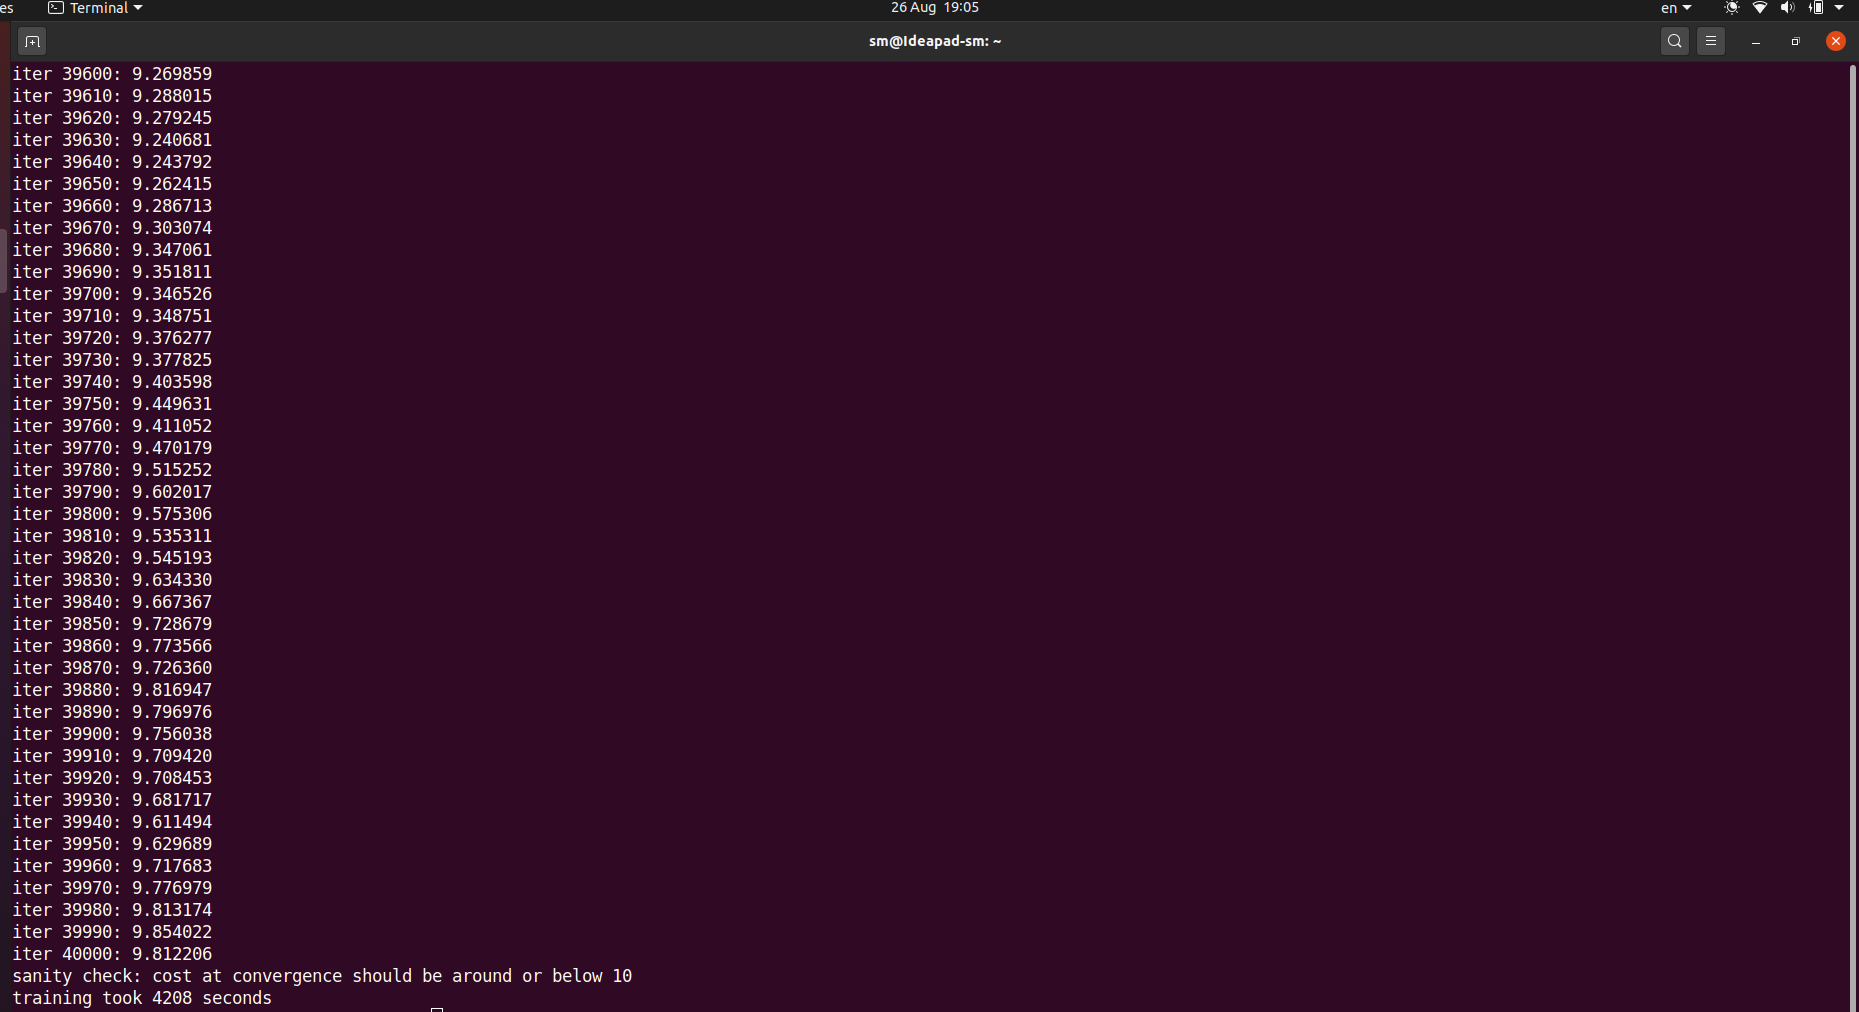
\includegraphics[scale=0.3]{results}
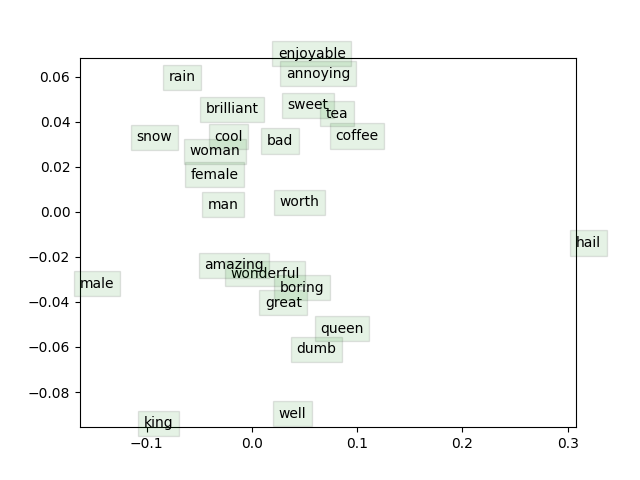
\includegraphics[scale=0.5]{word_vectors.png}
\end{document}

